\section{Gravity}
\begin{tabular*}{1.0\linewidth}{l|l}
  $M, m$ & masses of two bodies \\
  $r$    & distance between bodies
\end{tabular*}

Newton's law of gravity: the force between two bodies is $F = G\frac{Mm}{r^2}$, where $G$ is the
gravitational constant.

Units: since $[F] = \frac{LM}{T^2}$, we have $[G] = \frac{LM}{T^2}\frac{L^2}{M^2} = \frac{L^3}{MT^2}$.

\begin{tabular*}{1.0\linewidth}{l|l}
  $M_E = 5.972 \times 10^{24} kg$ & mass of the Earth \\
  $R =  6.371 \times 10^6 m$     & radius of the Earth \\
  $G = 6.67408 \times 10^{-11} m^3 kg^{-1} s^{-2}$        & gravitational constant\\
  $m$ & mass of an object
\end{tabular*}

The acceleration of the object due to gravity at the Earth's surface is
\begin{align*}
  g
  = \frac{F}{m}
  = G\frac{M_E}{R^2}
  = \frac{6.67408 \times 10^{-11} \times 5.972 \times 10^{24}}{(6.371 \times 10^6)^2}
  = 9.82 ms^{-2}.
\end{align*}


\section{Strategies for solving problems}
\subsection*{Units \& dimensional analysis}
\subsubsection*{}
\begin{mdframed}
  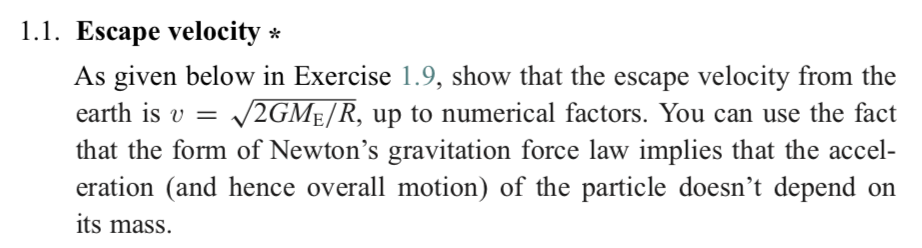
\includegraphics[width=400pt]{img/physics--classical-mechanics--morin--1-1.png}
\end{mdframed}

A projectile of mass $m$ is fired vertically upwards with velocity $v$ (no air-resistance).

When the projectile is at height $h$, the acceleration due to gravity is
$\frac{F}{m} = GM_E/(R + h)^2$, which does not depend on $m$.

We want units of $LT^{-1}$. We have

\begin{tabular*}{1.0\linewidth}{l|l}
  $[G]$        & $L^3M^{-1}T^{-2}$ \\
  $[M_E]$      & $M$ \\
  $[R]$        & $L$ \\
  $[GM_E / R]$ & $L^2T^{-2}$
\end{tabular*}

A quantity with the desired units is $\sqrt{GM_E/R}$.

More formally, suppose $v \propto G^iM_E^jR^k$.

Let  ${G, M_E, R}$ be a basis for a vector space.

Then the problem corresponds to the linear system
\begin{align*}
  \matMMMxNNN
  {3}{0}{1}
  {-1}{1}{0}
  {-2}{0}{0} \vecMMM{i}{j}{k} = \vecMMM{1}{0}{-1}.
\end{align*}
$i$ must be $1/2$, which implies $j = 1/2, k = -1/2$, i.e. $\sqrt{GM_E/R}$. \checkmark

\subsubsection*{}
\begin{mdframed}
  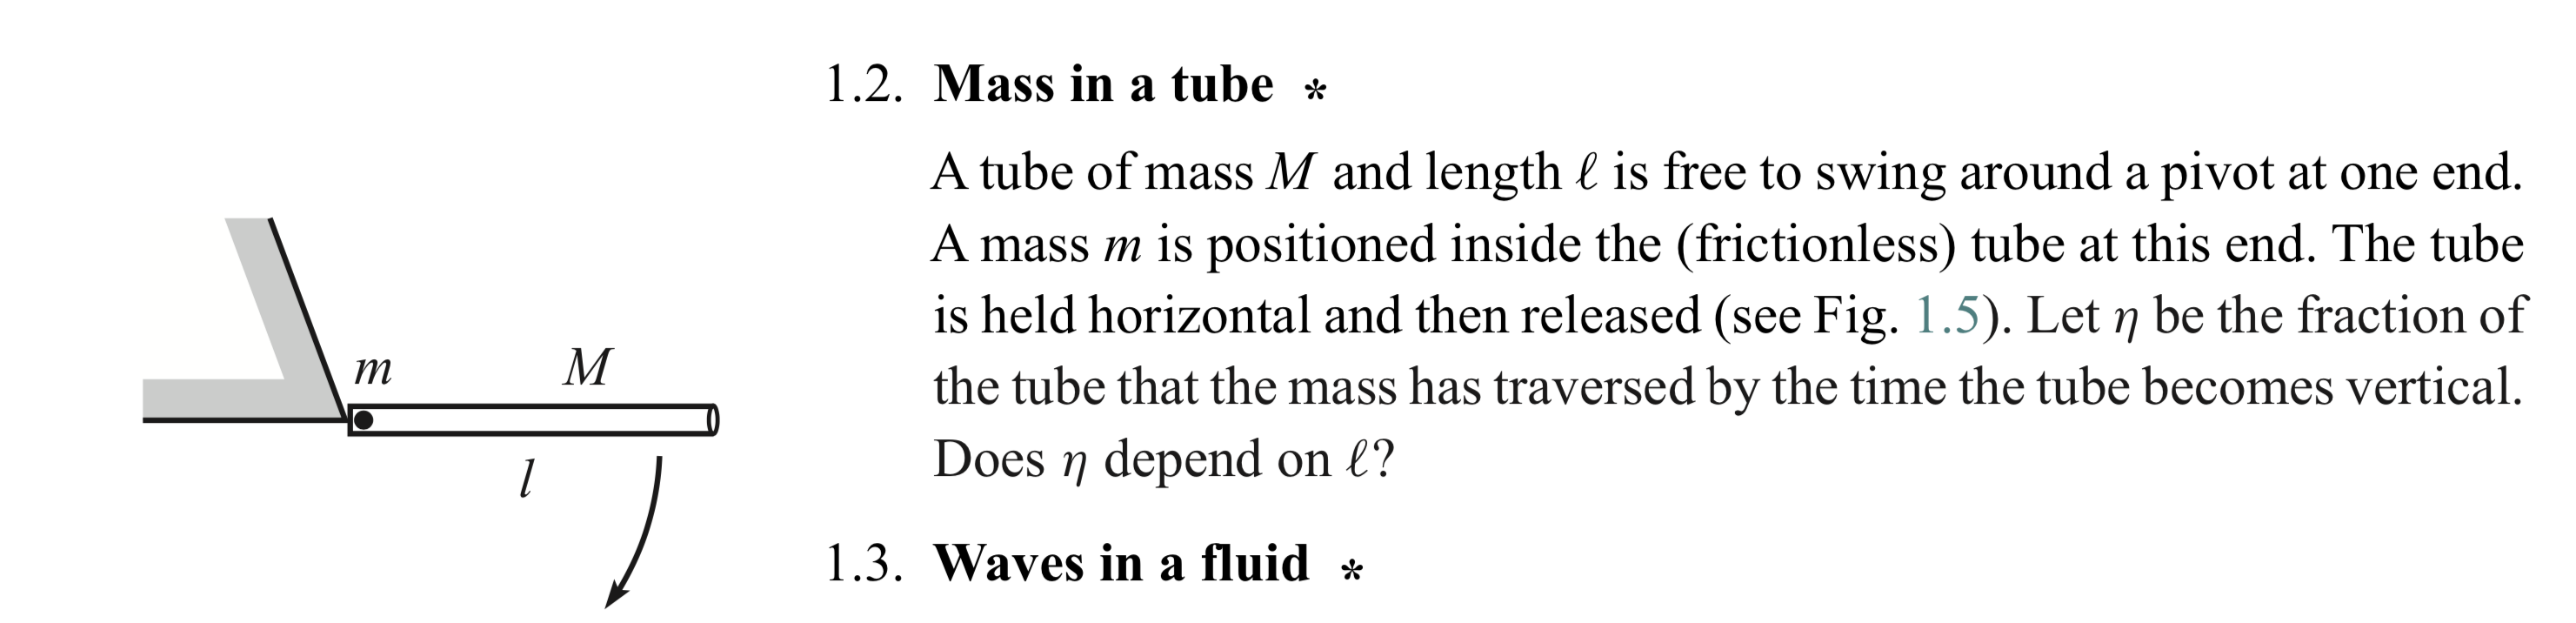
\includegraphics[width=400pt]{img/physics--classical-mechanics--morin--1-2.png}
\end{mdframed}

\begin{enumerate}
\item
  \begin{tabular}{l|l}
    $[l]$       & $L$ \\
    $[m], [M]$  & $M$ \\
    $[g]$       & $LT^{-2}$
  \end{tabular}\\
  As a fraction, $\eta$ is dimensionless. It cannot depend on $g$ since there is no other
  quantity to cancel out the time units. Suppose $\eta$ depends on some power of $l$. Then it must
  also depend on some other quantity involving distance. But there is no other
  such quantity. Therefore $\eta$ does not depend on $l$.  \checkmark

\item \todo{Why is this wrong?} We can choose an $l$ for which $\eta > 0$. Let $\eta^* > 0$ be such
  an $\eta$.

  However, as $l \to \infty$, we have $\eta \to 0$ since the distance traversed by the mass is bounded
  above by the distance the mass would drop under gravity with no opposing normal force from the tube;
  since $m$ is finite, this bound is finite.

  Therefore for all $\eta^* > 0$, we can choose an $l$ such that $\eta < \eta^*$. Therefore $\eta$
  does depend on $l$.
\end{enumerate}

\subsubsection*{}
\begin{mdframed}
  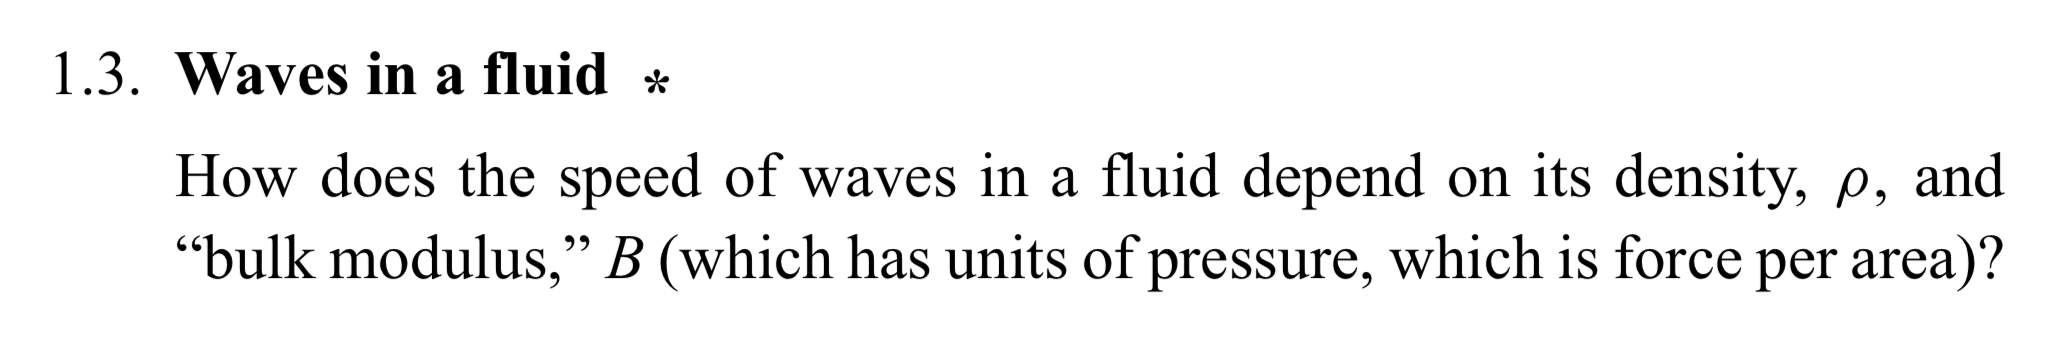
\includegraphics[width=400pt]{img/physics--classical-mechanics--morin--1-3.png}
\end{mdframed}

\begin{tabular}{l|l}
  speed   & $LT^{-1}$ \\
  density & $ML^{-3}$ \\
  bulk modulus & $MLT^{-2}L^{-2} = ML^{-1}T^{-2}$
\end{tabular}

\begin{align*}
  \matMMMxNN
  {-3}{-1}
  {1}{1}
  {0}{-2} \vecMM{i}{j} = \vecMMM{1}{0}{-1}.
\end{align*}
$\implies j = 1/2, i = -1/2$\\
So speed is proportional to $\sqrt{B/\rho}$. \checkmark

\subsubsection*{}
\begin{mdframed}
  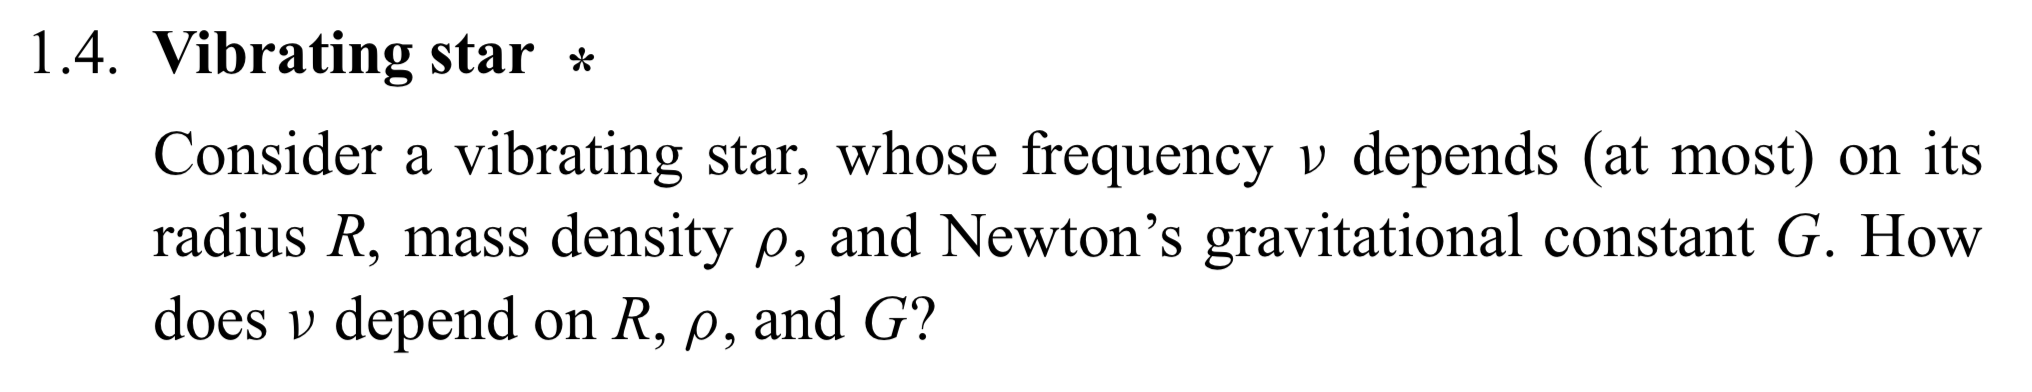
\includegraphics[width=400pt]{img/physics--classical-mechanics--morin--1-4.png}
\end{mdframed}
\begin{tabular}{l|l}
  Frequency $\nu$            & $T^{-1}$ \\
  Radius $R$                 & $L$ \\
  Mass density $\rho$        & $ML^{-3}$ \\
  Gravitational constant $G$ & $L^3M^{-1}T^{-2}$
\end{tabular}

Suppose $\nu \propto R^i\rho^jG^k$. Then $(i, j, k)^T$ would be a solution to
\begin{align*}
  \matMMMxNNN
  {1}{-3}{3}
  {0}{1}{-1}
  {0}{0}{-2} \vecMMM{i}{j}{k} = \vecMMM{0}{0}{-1}.
\end{align*}

$(0, 1/2, 1/2)$ is a solution, so frequency must be proportional to $\sqrt{G\rho}$. \checkmark

\subsubsection*{}
\begin{mdframed}
  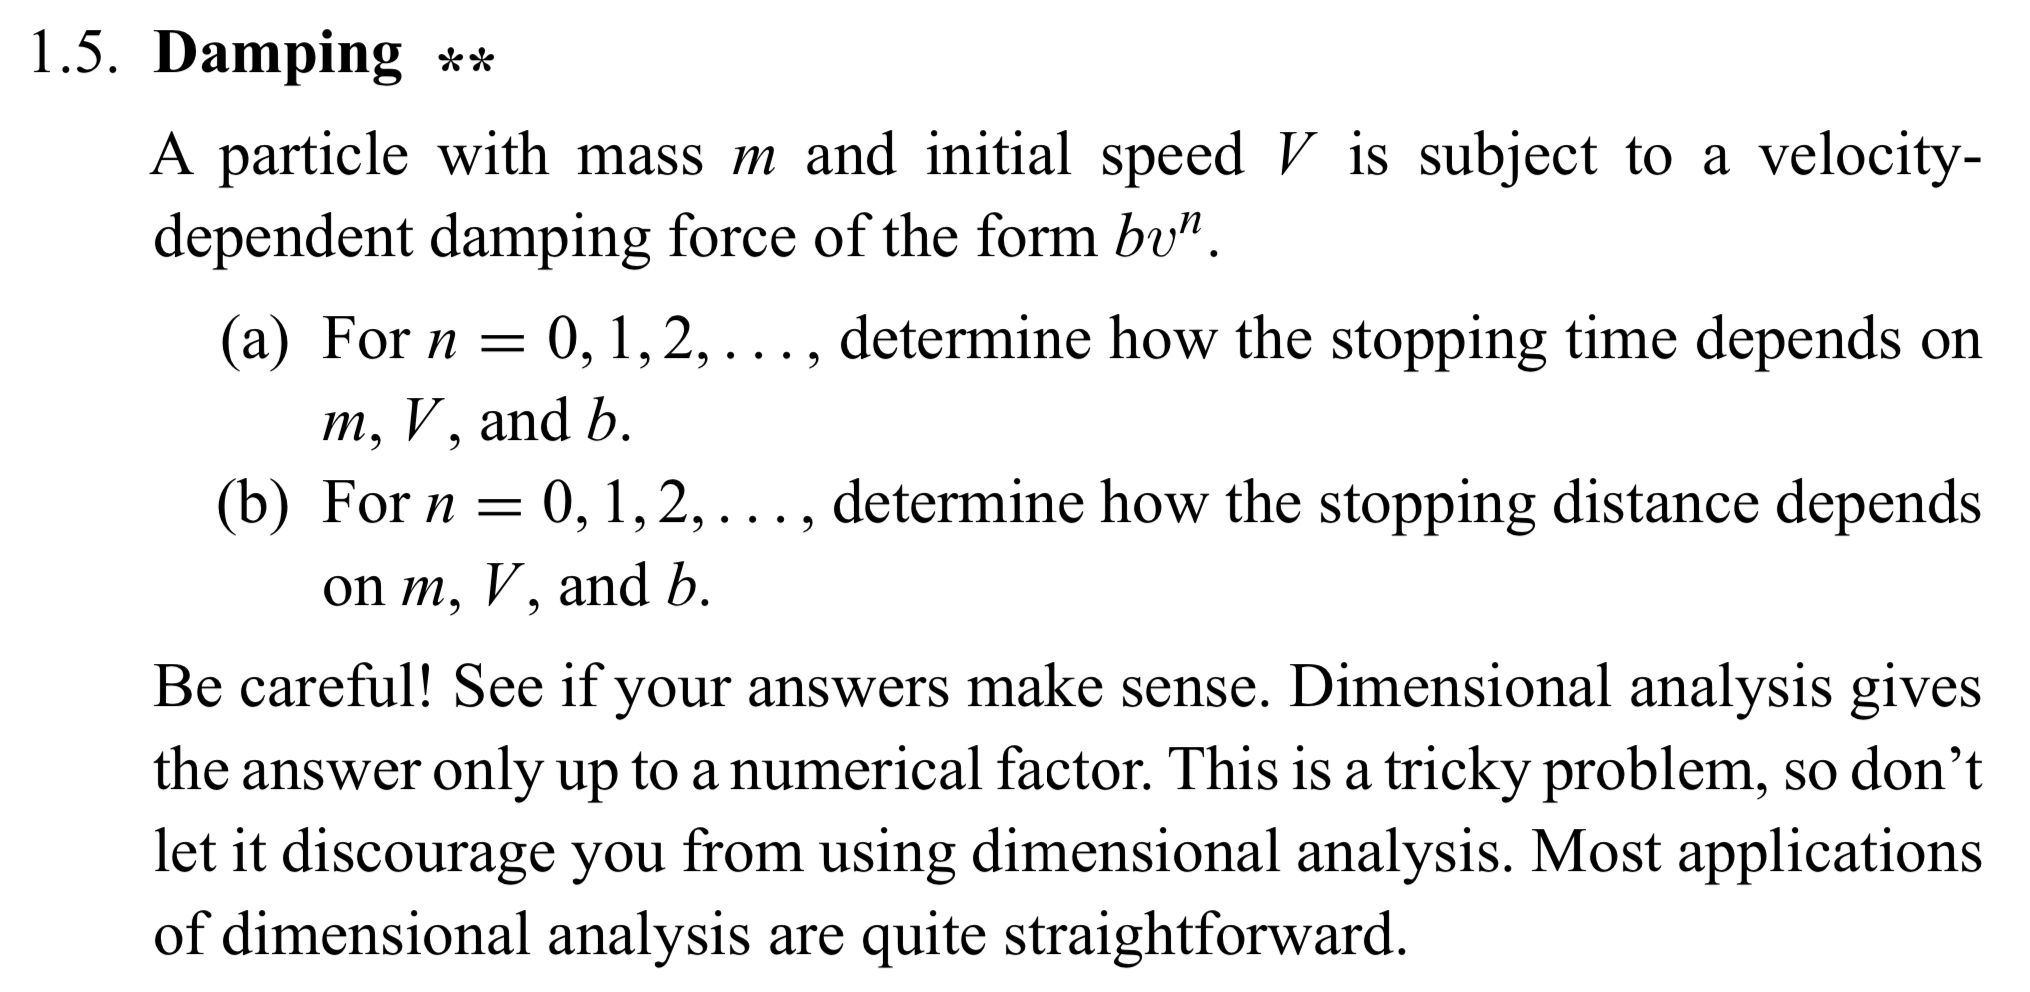
\includegraphics[width=400pt]{img/physics--classical-mechanics--morin--1-5.png}
\end{mdframed}

\begin{tabular}{l|l}
  Stopping time     & $T$ \\
  Stopping distance & $L$ \\
  \hline
  mass $m$          & $M$ \\
  Initial speed $V$ & $LT^{-1}$ \\
  Constant $b$      & $ML^{1-n}T^{n-2}$ \\
  \hline
  $v^n$             & $L^nT^{-n}$ \\
  Force $F = bv^n$  & $MLT^{-2}$
\end{tabular}

\begin{enumerate}[label=(\alph*)]
\item Stopping time\\
  Suppose $T \propto m^iV^jb^k$. Then
  \begin{align*}
    \matMMMxNNN
    {0}{1}{1-n}
    {1}{0}{1}
    {0}{-1}{n-2} \vecMMM{i}{j}{k} &= \vecMMM{0}{0}{1},
  \end{align*}
  so that
  \begin{align*}
    i + k &= 0 \\
    j + k(1 - n) &= 0 \\
    -j + k(n - 2) &= 1 \\
    k &= -1 \\
    i &= 1 \\
    j &= 1 - n.
  \end{align*}

\begin{verbatim}
#+begin_src mathematica :results pp
LinearSolve[{{0, 1, 1-n}, {1, 0, 1}, {0, -1, n-2}}, {0, 0, 1}]
#+end_src

#+RESULTS:
: {1, 1 - n, -1}
\end{verbatim}

  So we have
  \begin{align*}
    T \propto mV^{1 - n}/b.
  \end{align*}

  \begin{enumerate}
  \item $n = 0$\\
    $T \propto mV/b$. Makes sense.
  \item $n = 1$\\
    $T \propto m/b$. Why not dependent on $V$? Failure of dimensional analysis; dimensionless
    proportionality constant $f(n) = f(1) = \infty$.
  \item $n = 2$\\
    $T \propto m/(bV)$. Why decreasing with $V$? Again, $f(2) = \infty$.
  \end{enumerate}

\item Stopping distance\\
  Suppose $D \propto m^iV^jb^k$. Then
  \begin{align*}
    \matMMMxNNN
    {0}{1}{1-n}
    {1}{0}{1}
    {0}{-1}{n-2} \vecMMM{i}{j}{k} &= \vecMMM{1}{0}{0},
  \end{align*}
  so that
  \begin{align*}
    i + k &= 0 \\
    j + k(1 - n) &= 1 \\
    -j + k(n - 2) &= 0 \\
    k &= -1 \\
    i &= 1 \\
    j &= 2 - n.
  \end{align*}

\begin{verbatim}
#+begin_src mathematica :results pp
LinearSolve[{{0, 1, 1-n}, {1, 0, 1}, {0, -1, n-2}}, {1, 0, 0}]
#+end_src

#+RESULTS:
: {1, 2 - n, -1}
\end{verbatim}

  So we have
  \begin{align*}
    T \propto mV^{2 - n}/b.
  \end{align*}

  \begin{enumerate}
  \item $n = 0$\\
    $T \propto mV^2/b$. Makes sense.
  \item $n = 1$\\
    $T \propto mV/b$. Makes sense.
  \item $n = 2$\\
    $T \propto m/b$. Why not dependent on $V$?
  \end{enumerate}
\end{enumerate}

\subsection*{Approximations, limiting cases}

\subsubsection*{1.6}
\begin{mdframed}
  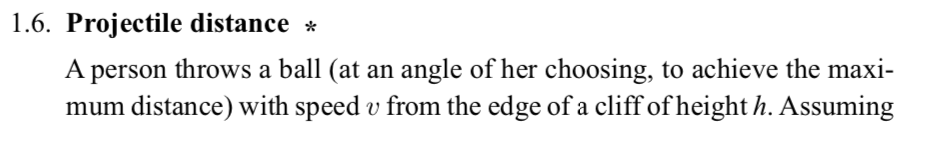
\includegraphics[width=400pt]{img/physics--classical-mechanics--morin--1-6-1.png}\\
  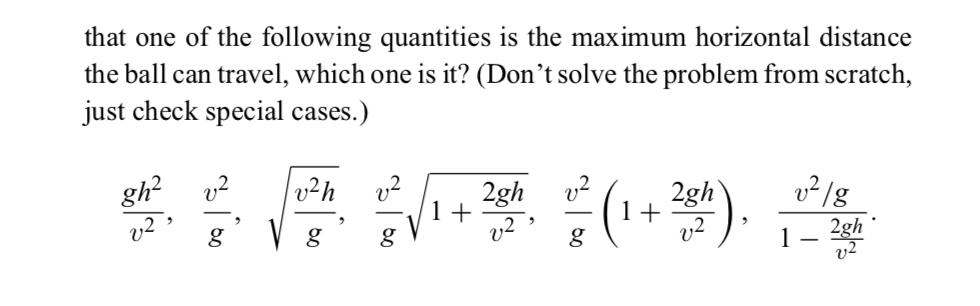
\includegraphics[width=400pt]{img/physics--classical-mechanics--morin--1-6-2.png}
\end{mdframed}

\begin{align*}
  [\frac{gh^2}{v^2}] &= \frac{L}{T^2} \frac{L^2}{1} \frac{T^2}{L^2} = L \checkmark \\
  [\frac{v^2}{g}]    &= \frac{L^2}{T^2} \frac{T^2}{L} = L \checkmark
\end{align*}

...

\subsubsection*{}
\begin{mdframed}
  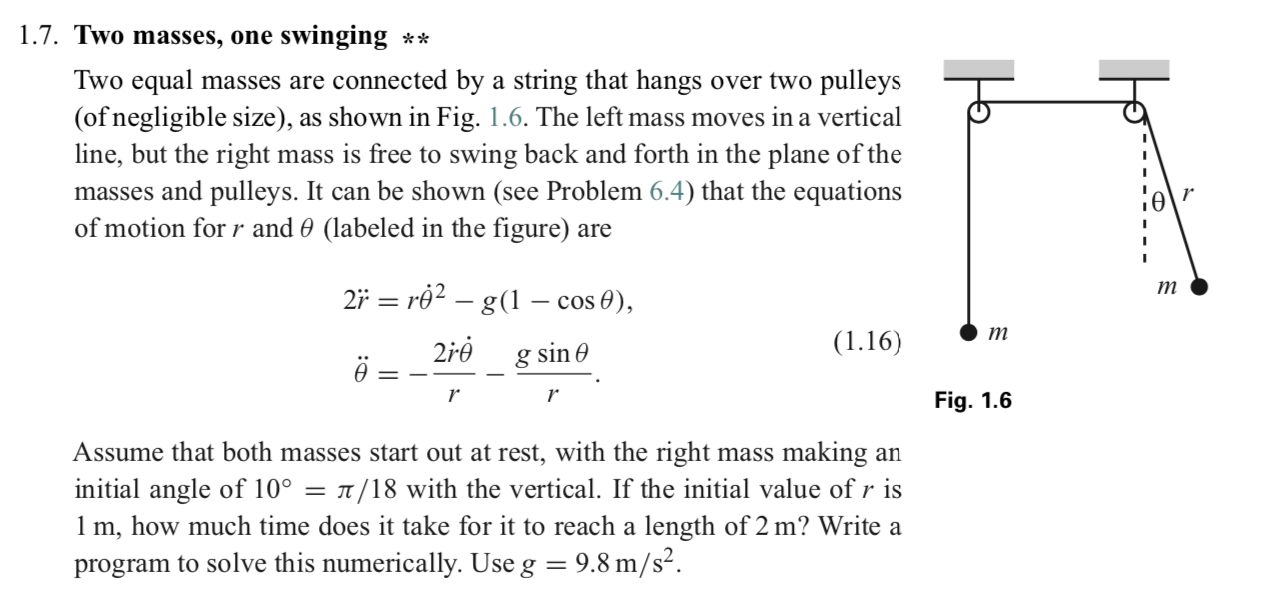
\includegraphics[width=400pt]{img/physics--classical-mechanics--morin--1-7.png}
\end{mdframed}

\begin{minted}{python3}
from dataclasses import dataclass
from math import cos
from math import pi
from math import sin

g = 9.8   # acceleration due to gravity (m/s)
dt = 0.0001  # tick interval (s)

@dataclass
class World:
    r: float = 1
    r_dot: float = 0
    theta: float = pi / 18
    theta_dot: float = 0
    time: float = 0

def r_dot_dot(self):
    return 0.5 * (self.r * self.theta_dot**2 - g*(1 - cos(self.theta)))

def theta_dot_dot(self):
    return -2 * self.r_dot * self.theta_dot / self.r - g * sin(self.theta) / self.r

def tick(self):
    self.r_dot += dt * self.r_dot_dot()
    self.r += dt * self.r_dot
    self.theta_dot += dt * self.theta_dot_dot()
    self.theta += dt * self.theta_dot
    self.time += dt


def main():
    world = World()
    while world.r < 2:
        world.tick()

    print(world.time)
\end{minted}

\section{Statics}
\subsection*{Balancing forces}
\subsubsection*{}
\begin{mdframed}
  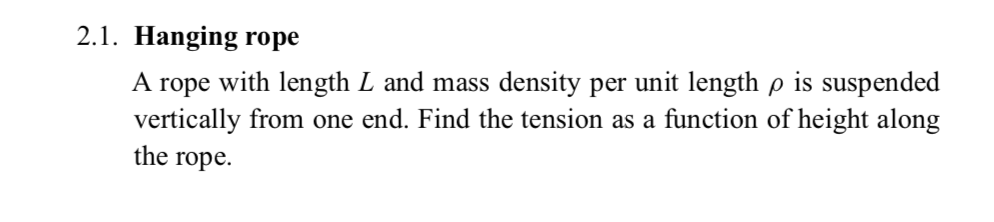
\includegraphics[width=400pt]{img/physics--classical-mechanics--morin--2-1.png}
\end{mdframed}

Let $h$ be height measured from the free (lower) end. The tension $F$ is due to the weight of the
section of the rope below:
\begin{align*}
  F = \rho hg,
\end{align*}
for $0 \leq h \leq L$. \checkmark

\begin{mdframed}
  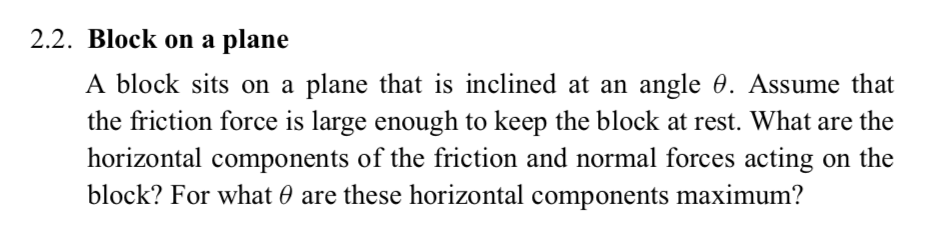
\includegraphics[width=400pt]{img/physics--classical-mechanics--morin--2-2.png}
\end{mdframed}

The normal force (component of weight normal to surface) is $mg\cos\theta$. The horizontal component
of this is $mg\cos\theta\sin\theta$.

Equivalently, the friction force (component of weight along surface) is $mg\sin\theta$. The
horizontal component of this is $mg\sin\theta\cos\theta$.

These are presumably maximum at $\theta = \pi/4$. \checkmark

\newpage
\begin{mdframed}
  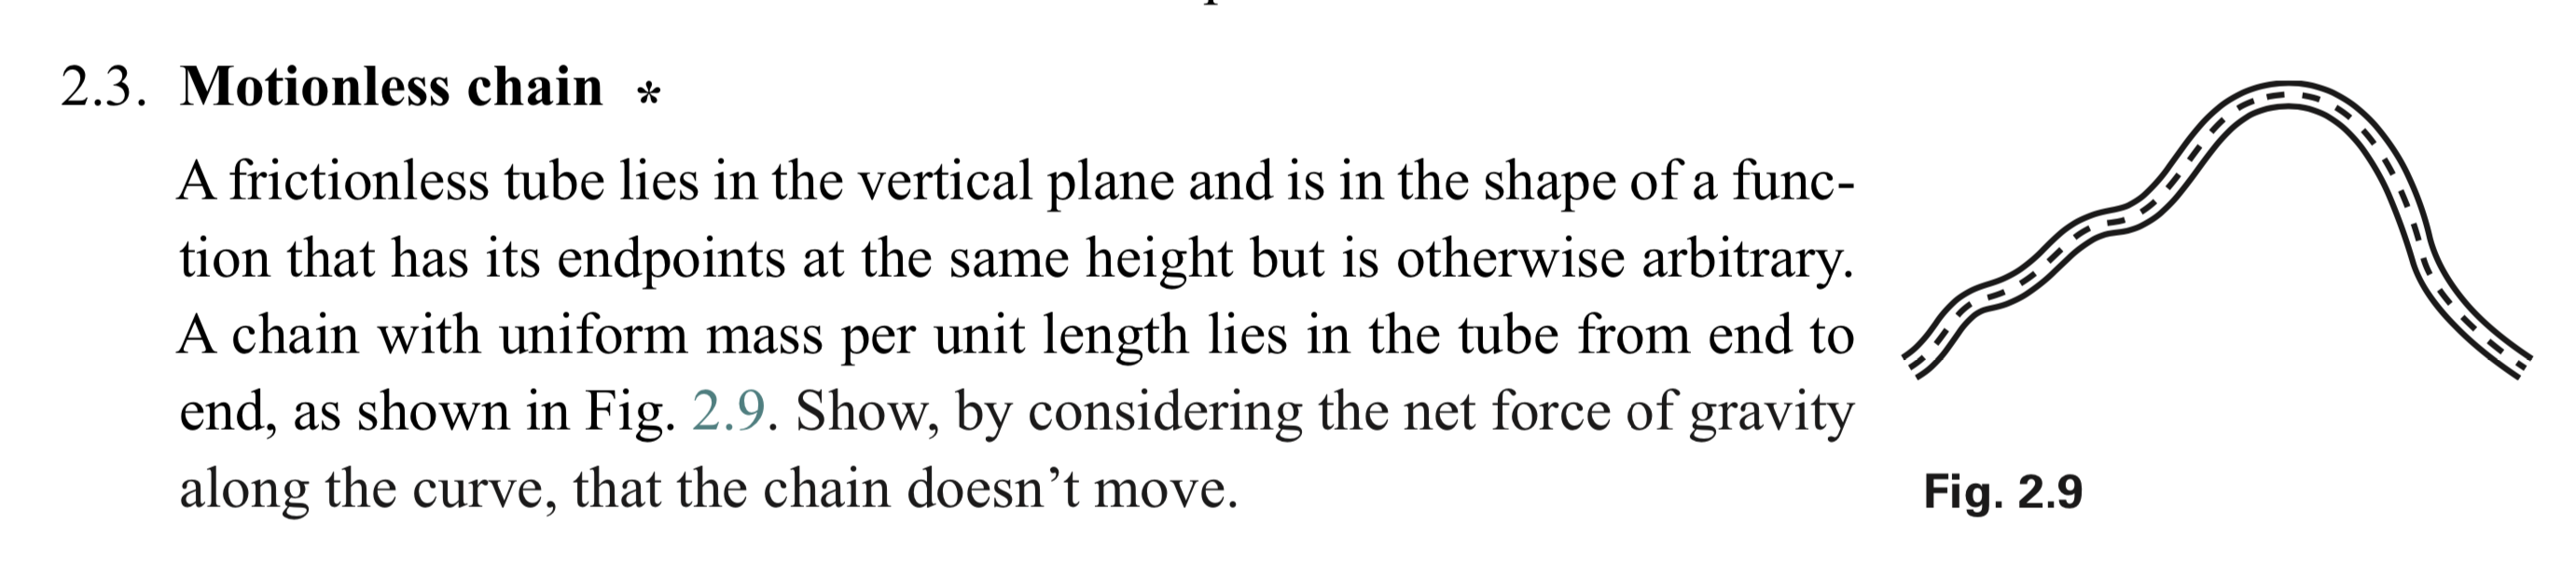
\includegraphics[width=400pt]{img/physics--classical-mechanics--morin--2-3.png}
\end{mdframed}

Focus on an arbitrary point $x$ along the horizontal axis. The height of the chain at this point is
$y(x)$ with tangent slope $\tan \theta = y'(x)$. Consider a short section of chain of length
$\dl = \sqrt{\dx^2 + \dy^2} = \sqrt{1 + \tan^2\theta} \dx$. Let the mass per unit length be
$\rho$. The weight is $\rho (\dl) g$ downwards. This has a component normal to the chain which is
irrelevant, since it is balanced by the opposing normal force from the fixed tube. The component of
weight along the chain is $\rho (\dl) g \sin\theta$.

There will be tension and normal (compression) forces acting to oppose this component of weight, but
we don't need to analyse these. Instead we ask what the net force $F$ is on the system. Let $L$ be
the total length of the chain. We have

\begin{align*}
  F &= \int_{l=0}^{l=L} \rho g \sin\theta \dl \\
    &= \rho g \int_{l=0}^{l=L} \sin\theta \sqrt{1 + \tan^2\theta} \dx.
\end{align*}
Note that $\sin\theta = \frac{\tan\theta}{\sqrt{1 + \tan^2\theta}}$, and that $\tan\theta =
\dydx$. Therefore
\begin{align*}
  F &= \rho g \int_{l=0}^{l=L} \dy\\
    &= \rho g \(y(L) - y(0)\)\\
    &= 0.
\end{align*}

\newpage
\begin{mdframed}
  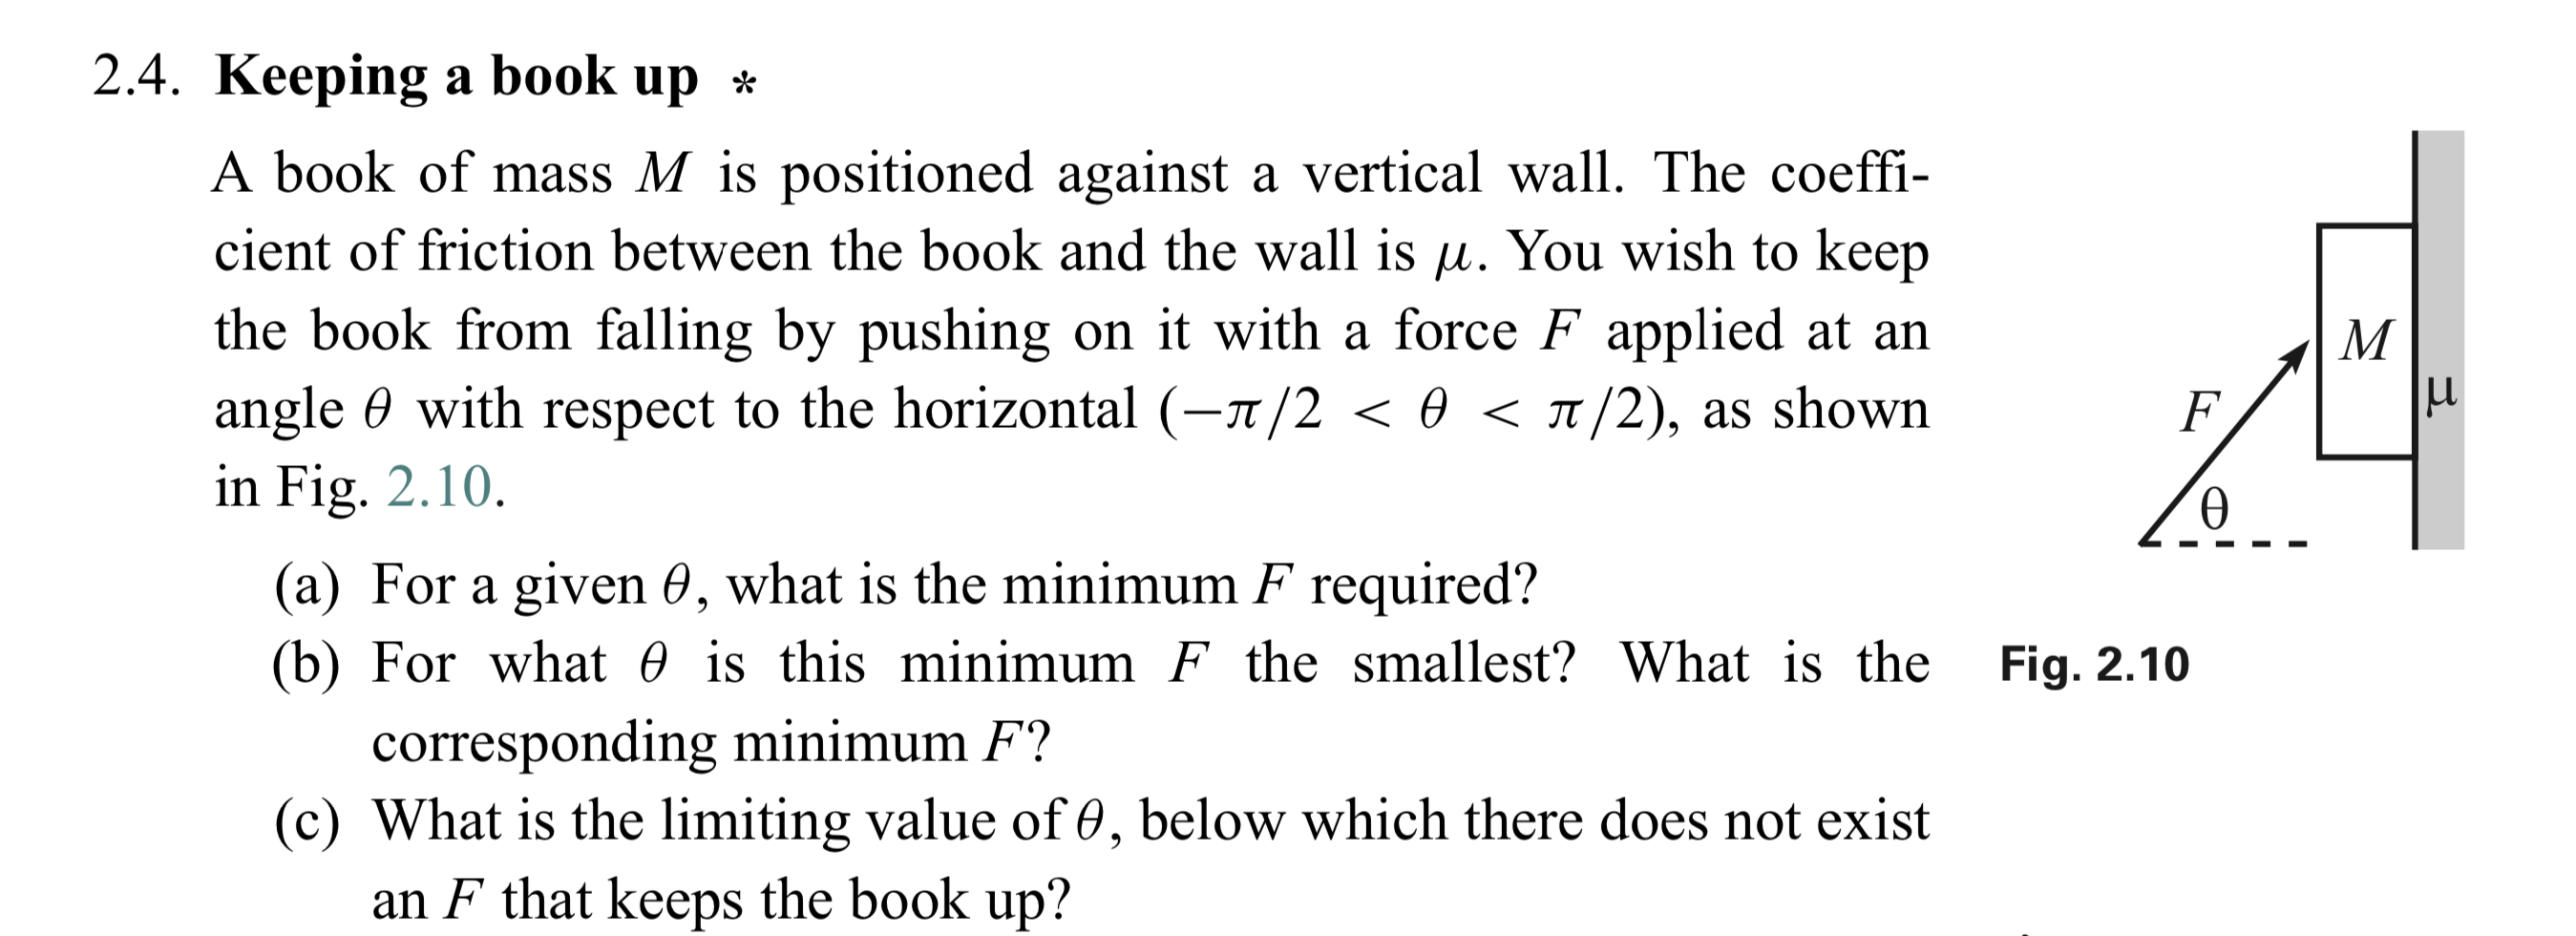
\includegraphics[width=400pt]{img/physics--classical-mechanics--morin--2-4.png}
\end{mdframed}

When $F = 0$, the book will fall down freely under the gravity force $Mg$.

The relevant forces are
\begin{itemize}
\item the book weight $Mg$,
\item an upwards supporting force of $S = F\sin\theta$ (which will be negative when $\theta < 0$,
  i.e. when $F$ is pointing downwards),
\item a normal force of $N = F\cos\theta$.
\end{itemize}

So, there is a downwards force of $D = W - S$. And therefore there is also an upwards friction force
of $\min\(\mu N, D\)$. When this is less than $D$, the book is sliding down.

Suppose $\theta$ is positive and $F$ is initially holding the book in place. This means that
$\mu N > D$. As $F$ decreases, it causes $S$ to decrease, which means that $D$ increases. At the
same time, $\mu N$ is decreasing. So $D$ and $\mu N$ are moving towards each other. When they meet,
the book is about to start sliding down.

\begin{enumerate}[label=(\alph*)]
\item The minimum $F$ occurs when $D = \mu N$. I.e.
  \begin{align*}
    W - S            &= \mu N \\
    Mg - F\sin\theta &= \mu F\cos\theta \\
    F &= \frac{Mg}{\sin\theta + \mu\cos\theta}.
  \end{align*}
  Makes sense: more force needed if book heavier; less force needed if $\mu$ larger ($\cos$ is
  positive in $(-\pi/2, \pi/2)$); \todo{change with $\theta$}.
\item We seek the $\theta \in (-\pi/2, \pi/2)$ which maximizes
  $g(\theta) = \sin\theta + \mu\cos\theta$. We have $g'(\theta) = \cos\theta - \mu\sin\theta$, and
  setting this equal to zero gives $\tan\theta = 1/\mu$. So, the minimum $F$ is smallest for
  $\theta = \tan^{-1}(1/\mu)$. This minimum $F$ is (using $\cos\theta = 1/\sqrt{1 + \tan^2\theta}$)
  \begin{align*}
    F
    &= \frac{Mg/\cos\theta}{\tan\theta + \mu} \\
    &= \frac{Mg\sqrt{1 + \tan^2\theta}}{\tan\theta + \mu} \\
    &= \frac{Mg\sqrt{1 + 1/\mu^2}}{1/\mu + \mu}.
  \end{align*}

  \todo{Book gives $\frac{Mg}{\sqrt{1 + \mu^2}}$}

\begin{verbatim}
#+begin_src mathematica :results raw pp
Simplify[Sqrt[1 + 1/mu^2]/(1/mu + mu)]
#+end_src

#+RESULTS:
: (Sqrt[1 + mu^(-2)]*mu)/(1 + mu^2)

\end{verbatim}

\item As $\theta$ decreases below zero, $D$ increases ($S$ is now negative) and $\mu N$
  decreases. The limiting...\todo{TODO}
\end{enumerate}
\newpage
\section{Using $F = ma$}
\subsection*{Free-body diagrams}
\subsubsection*{}
\begin{mdframed}
  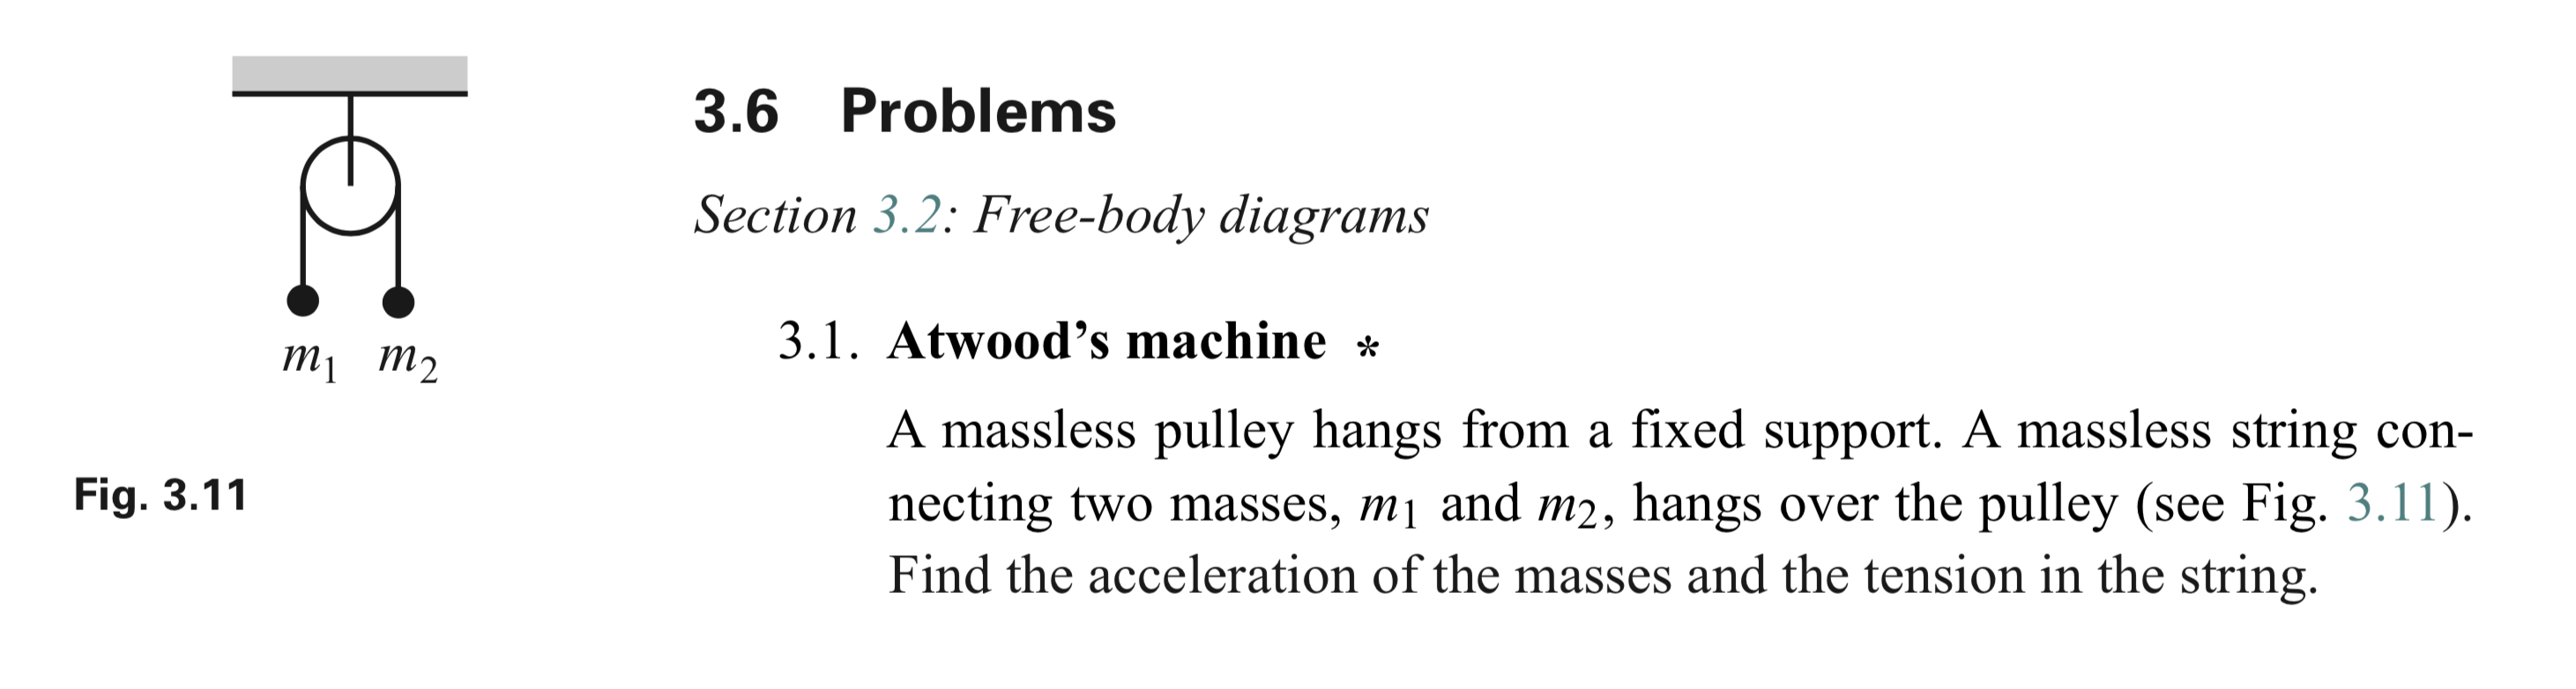
\includegraphics[width=400pt]{img/physics--classical-mechanics--morin--3-1.png}
\end{mdframed}
Let $a$ be the rightward acceleration of the string, and $T$ be the tension in the string.

To find $a$ is simple: there is a net force of $F = m_2g - m_1g$, therefore
\begin{align}
  a = \frac{F}{m} = \frac{m_2g - m_1g}{m_1 + m_2}. \label{morin-3-1-a} \checkmark
\end{align}
However, this doesn't give $T$.

Below are two ways to find $T$ by using $F = ma$ at each mass:
\begin{enumerate}
\item by substituting the above expression for $a$ into either one of them,
\item by solving the two jointly as a linear system, without using the above expression for $a$.
\end{enumerate}

So it seems that the acceleration of the whole system can be found using ``one degree of
freedom''(?), but that finding the tension requires solving a two-dimensional linear system.

Using $F = ma$ at each mass, we have
\begin{align}
  m_1a &= T-m_1g   \label{morin-3-1-Fma1}\\
  m_2a &= m_2g - T \label{morin-3-1-Fma2}.
\end{align}
From \eqref{morin-3-1-a} and \eqref{morin-3-1-Fma1} we have
\begin{align*}
  T &= \frac{m_1(m_2g - m_1g)}{m_1 + m_2} + m_1g \\
    &= \frac{2m_1m_2g}{m_1 + m_2}. \checkmark
\end{align*}
And as a check, from \eqref{morin-3-1-a} and \eqref{morin-3-1-Fma2} we have
\begin{align*}
  T &= m_2g - \frac{m_2(m_2g - m_1g)}{m_1 + m_2} \\
    &= \frac{2m_1m_2g}{m_1 + m_2}.
\end{align*}

Alternatively, we can solve the linear system given by $F = ma$ at each mass:
\begin{align*}
  m_1a - T &= -m_1g \\
  m_2a + T &= m_2g,
\end{align*}
i.e.
\begin{align*}
  \mat{m_1}{-1}
      {m_2}{1} \vecMM{a}{T} = \vecMM{-m_1g}{m_2g}.
\end{align*}
Solution:
\begin{align*}
    T = m_1a + m_1g &= m_2g - m_2a \\
    a &= \frac{m_2g - m_1g}{m_1 + m_2}.
\end{align*}
